\documentclass[12pt,a4paper,openright]{report}
\usepackage[legalpaper, portrait, margin=1.2in]{geometry}
\usepackage[utf8]{inputenc}
\usepackage[italian]{babel}
\usepackage{fancyhdr}
\usepackage{graphicx}
\usepackage{hyperref}
% \usepackage{soul,xcolor}
% \usepackage{soul}
\usepackage{xcolor}
\usepackage[normalem]{ulem}
\usepackage{caption}
\usepackage{listings}
\usepackage{subfig}
\usepackage{mwe}

\lstset{basicstyle=\small\ttfamily}

\pagenumbering{arabic}   


\title{PCD: Elaborato due}
\author{Bachetti Michele, Marcantognini Elia, Tinti Angelo}
\date{Aprile - Maggio 2022}

\begin{document}

% Line strike through color
% \setstcolor{red}

\maketitle

\tableofcontents

\chapter*{Introduzione}
\addcontentsline{toc}{chapter}{Introduzione}

L'elaborato presentato in questo report è composto di più parti:
\begin{itemize}
    \item nella prima parte, si implementa una versione asincrona del progetto realizzato nel \href{https://github.com/eliamarcantognini/pcd2122_ass1/blob/master/doc/report.pdf}{primo elaborato};
    \item nella seconda parte, si ...;
    \item nella terza parte, si ....
\end{itemize}

Per visualizzare il codice sono presenti i repository su GitHub:
\begin{itemize}
    \item \href{https://github.com/eliamarcantognini/pcd2122_ass1/tree/ass2-tasks}{Primo esercizio} alla pagina \url{https://github.com/eliamarcantognini/pcd2122_ass1/tree/ass2-tasks};
    \item \href{https://github.com/eliamarcantognini/pcd2122_ass2es2}{Secondo esercizio} alla pagina \url{https://github.com/eliamarcantognini/pcd2122_ass2es2};
    \item \href{https://github.com/eliamarcantognini/pcd2122_ass2es2}{Terzo esercizio} alla pagina \url{https://github.com/eliamarcantognini/pcd2122_ass2es2}.
\end{itemize}


\chapter{Primo esercizio} 
\label{chapter:es1}
\section{Strategia Risolutiva}

Per la realizzazione del primo punto seguendo, un approccio a task, si è deciso di mantenere lo scheletro principale realizzato nel \href{https://github.com/eliamarcantognini/pcd2122_ass1/blob/master/doc/report.pdf}{primo elaborato} (\url{https://github.com/eliamarcantognini/pcd2122_ass1/blob/master/doc/report.pdf}) andando a modificare solo quelle componenti non necessarie.

Come da specifiche la soluzione implementata è basata sui Java Executors per la gestione dei Task da completare in parallelo.
%
In particolare, si è pensato ad un singolo Task che specifica le operazioni da effettuare per l'aggiornamento delle informazioni di uno specifico corpo ad ogni iterazione.

Il modello pensato riflette l'insieme di istruzioni che nel precedente \textit{assignment} erano affidate agli agenti e per questo motivo è realizzato senza la necessità di dover restituire alcun risultato, aspetto che semplifica la gestione dei Task in quanto non esistono singoli risultati da dover ricomporre.

Seguendo questa idea viene creato un Task per ogni corpo nella simulazione, da assegnare ad un Java Executor che si occuperà della sua esecuzione.

Una volta terminata l'esecuzione di tutti i Task viene aggiornata la view in modo da rispettare il requisito di coerenza tra ciò che viene mostrato all'utente e lo stato del programma.

\section{Architettura e implementazione}
\label{section:arch_impl}

\subsection{Simulator}
\label{subs:simulator}

Simulator rispetto l'assignement precedente è stato modificato affinché implementasse un approccio a task. La parte più importante si trova dentro il metodo \texttt{exec()} il quale gestisce le iterazioni della simulazione e manda in esecuzione i task sfruttando le classi \texttt{Executors} e \texttt{ExecutorService} che abbiamo visto a lezione. \texttt{startSimulation} permette di avviare l'\texttt{exec} e sfrutta un thread differente affinché non venga bloccato il sistema.
\newline
I task vengono mandati in esecuzione sui singoli corpi e una volta avviati se ne attende il completamento.
\newline
Non è più presente una \texttt{CyclicBarrier} per la sincronizzazione dei thread al termine delle iterazioni, ma per il medesimo scopo viene utilizzato \texttt{\nameref{subs:task_sync_m}} che viene aggiornato dagli \texttt{\nameref{subs:update_task}}. Quando il monitor permette di proseguire viene aggiornato il sistema\footnote{Come nell'assignment precedente, vengono aggiornate le due liste, usate per le letture e le scritture, aumentato il tempo virtuale e aggiornata la view.} e si prosegue all'iterazione successiva.
% \newline
% Come metodo di esecuzione dell'Executor è stato scelto \texttt{newFixedThreadPool} visto a lezione.

\subsection{UpdateTask}
\label{subs:update_task}

Rappresenta il singolo modello di Task presente nel sistema e contiene le istruzioni per poter aggiornare un singolo corpo ad una iterazione.

Corrisponde quasi completamente al comportamento racchiuso all'interno degli Agenti realizzati nel primo \textit{assignment}, per cui le peculiarità sono le stesse.

Ciò che fa in più è il dover segnalare di aver completato le sue operazione al \texttt{TaskSyncMonitor} per potersi coordinare con gli altri Task.

\subsection{SyncMonitor}
\label{subs:sync_m}

Monitor utilizzato per le modifiche e controlli relativi al fatto che la simulazione possa continuare o meno. Il valore al suo interno viene modificato quando nell'interfaccia grafica viene premuto il tasto ``\texttt{STOP}" e il controllo viene effettuato da \texttt{Simulator} all'inizio di ogni nuova iterazione.

\subsection{TaskSyncMonitor}
\label{subs:task_sync_m}

Monitor usato per sincronizzare la terminazione dei task affinché si proceda alla successiva iterazione della simulazione solamente quando tutti hanno aggiornato le nuove posizioni dei corpi.
%
In particolare una volta creato l'\textit{executor} e avergli assegnato i task da completare ci si mette in attesa della loro terminazione chiamando l'istruzione \textit{wait()} sul monitor.
%
I singoli task, prima di terminare la loro esecuzione, si preoccupano di aumentare il contatore all'interno di \texttt{TaskSyncMonitor} prima della loro terminazione e, se è l'ultimo Task ad aver completato, risvegliare il Thread che era in attesa.

Al termine di ogni iterazione il contatore viene resettato per poter riutilizzare il monitor nell'iterazione successiva.


\section{Verifica delle prestazioni} \label{section:prestazioni}

Nella presente sezione si analizzeranno le prestazioni confrontando le performance di quattro modelli, i primi tre modelli già discussi nel \href{https://github.com/eliamarcantognini/pcd2122_ass1/blob/master/doc/report.pdf}{precedente elaborato} (\url{https://github.com/eliamarcantognini/pcd2122_ass1/blob/master/doc/report.pdf}) e il nuovo modello asincrono:
\begin{itemize}
    \item \textit{Sequenziale}, il modello in cui non è implementato il multithreading;
    \item \textit{1:1}, il modello in cui è implementato un mapping uno a uno tra numero di corpi e numero di thread;
    \item \textit{Fixed Thread}, il modello in cui il numero di thread è pari al numero di core utilizzabili dall'applicazione;
    \item \textit{Async}, il modello implementato mediante l'approccio a task.
\end{itemize}

L'analisi delle prestazioni è stata eseguita confrontando le performance dei quattro modelli implementati ed ognuno di loro è stata testato su un numero variabile di corpi e iterazioni.

Analizzando in dettaglio i risultati riportati nella Tabella ~\ref{tab:perf}, è possibile calcolare l'incremento della velocità di esecuzione dei vari modelli a confronto, trascurando i risultati ottenuti con il parametro \textit{nBodies} pari a 100 poiché poco significativi nell'analisi della scalabilità dell'applicazione.

Confrontando il nuovo modello \textit{Async}, si può notare come esso sia nettamente migliore dei modelli \textit{Sequenziale} e \textit{1:1} e come vada  più veloce anche del modello \textit{Fixed Thread}, con un incremento della velocità di computazione di circa il 20\%.
L'implementazione asincrona risulta quindi la più veloce nonostante abbia un andamento del tutto analogo a quella del modello \textit{Fixed Thread}. Ciò è dovuto all'implementazione degli \textit{executors} e al minor \textit{overhead}\footnote{https://www.researchgate.net/publication/2609854\_A\_Java\_ForkJoin\_Framework}\footnote{https://www.oracle.com/technical-resources/articles/java/fork-join.html} rispetto alla gestione dei thread classica.

\begin{table}[ht]
    \centering
    \begin{tabular}{|c|c|c|c|c|c|}
        \hline
        \multicolumn{2}{|c|}{Parametri} & \multicolumn{4}{|c|}{Risultati dei modelli in secondi} \\
        \hline
        N° corpi & N° iterazioni & Sequenziale & 1:1 & Fixed Thread & Async \\
        \hline
        & 1000 & 0.083 & 0.956 & 0.152 & 0.155 \\
        100 & 10000 & 0.686 & 8.874 & 0.805 & 0.860 \\
        & 50000 & 2.465 & 44.897 & 3.646 & 3.749 \\
        \hline
        & 1000 & 7.145 & 10.572 & 1.716 & 1.431 \\
        1000 & 10000 & 72.094 & 109.132 & 16.680 & 13.589 \\
        & 50000 & 359.054 & 527.608 & 83.070 & 67.392 \\
        \hline
        & 1000 & 175.565 & 58.198 & 38.800 & 32.072 \\
        5000 & 10000 & 1477.274 & 578.232 & 458.425 & 313.677 \\
        & 50000 & 9271.029 & 2897.990 & 1973.932 & 1559.505 \\
        \hline
    \end{tabular}
    \caption{Tabella riassuntiva delle misurazioni.}
    \label{tab:perf}
\end{table}

Nelle Figure ~\ref{fig:iterations} e ~\ref{fig:bodies} sono visibili i grafici dei quattro modelli messi a confronto con numeri variabili di iterazioni e corpi.

\begin{figure}[ht]
    \begin{center}
        \begin{minipage}{.5\linewidth}
            \centering
            \subfloat[]{\label{stats_iterations:a}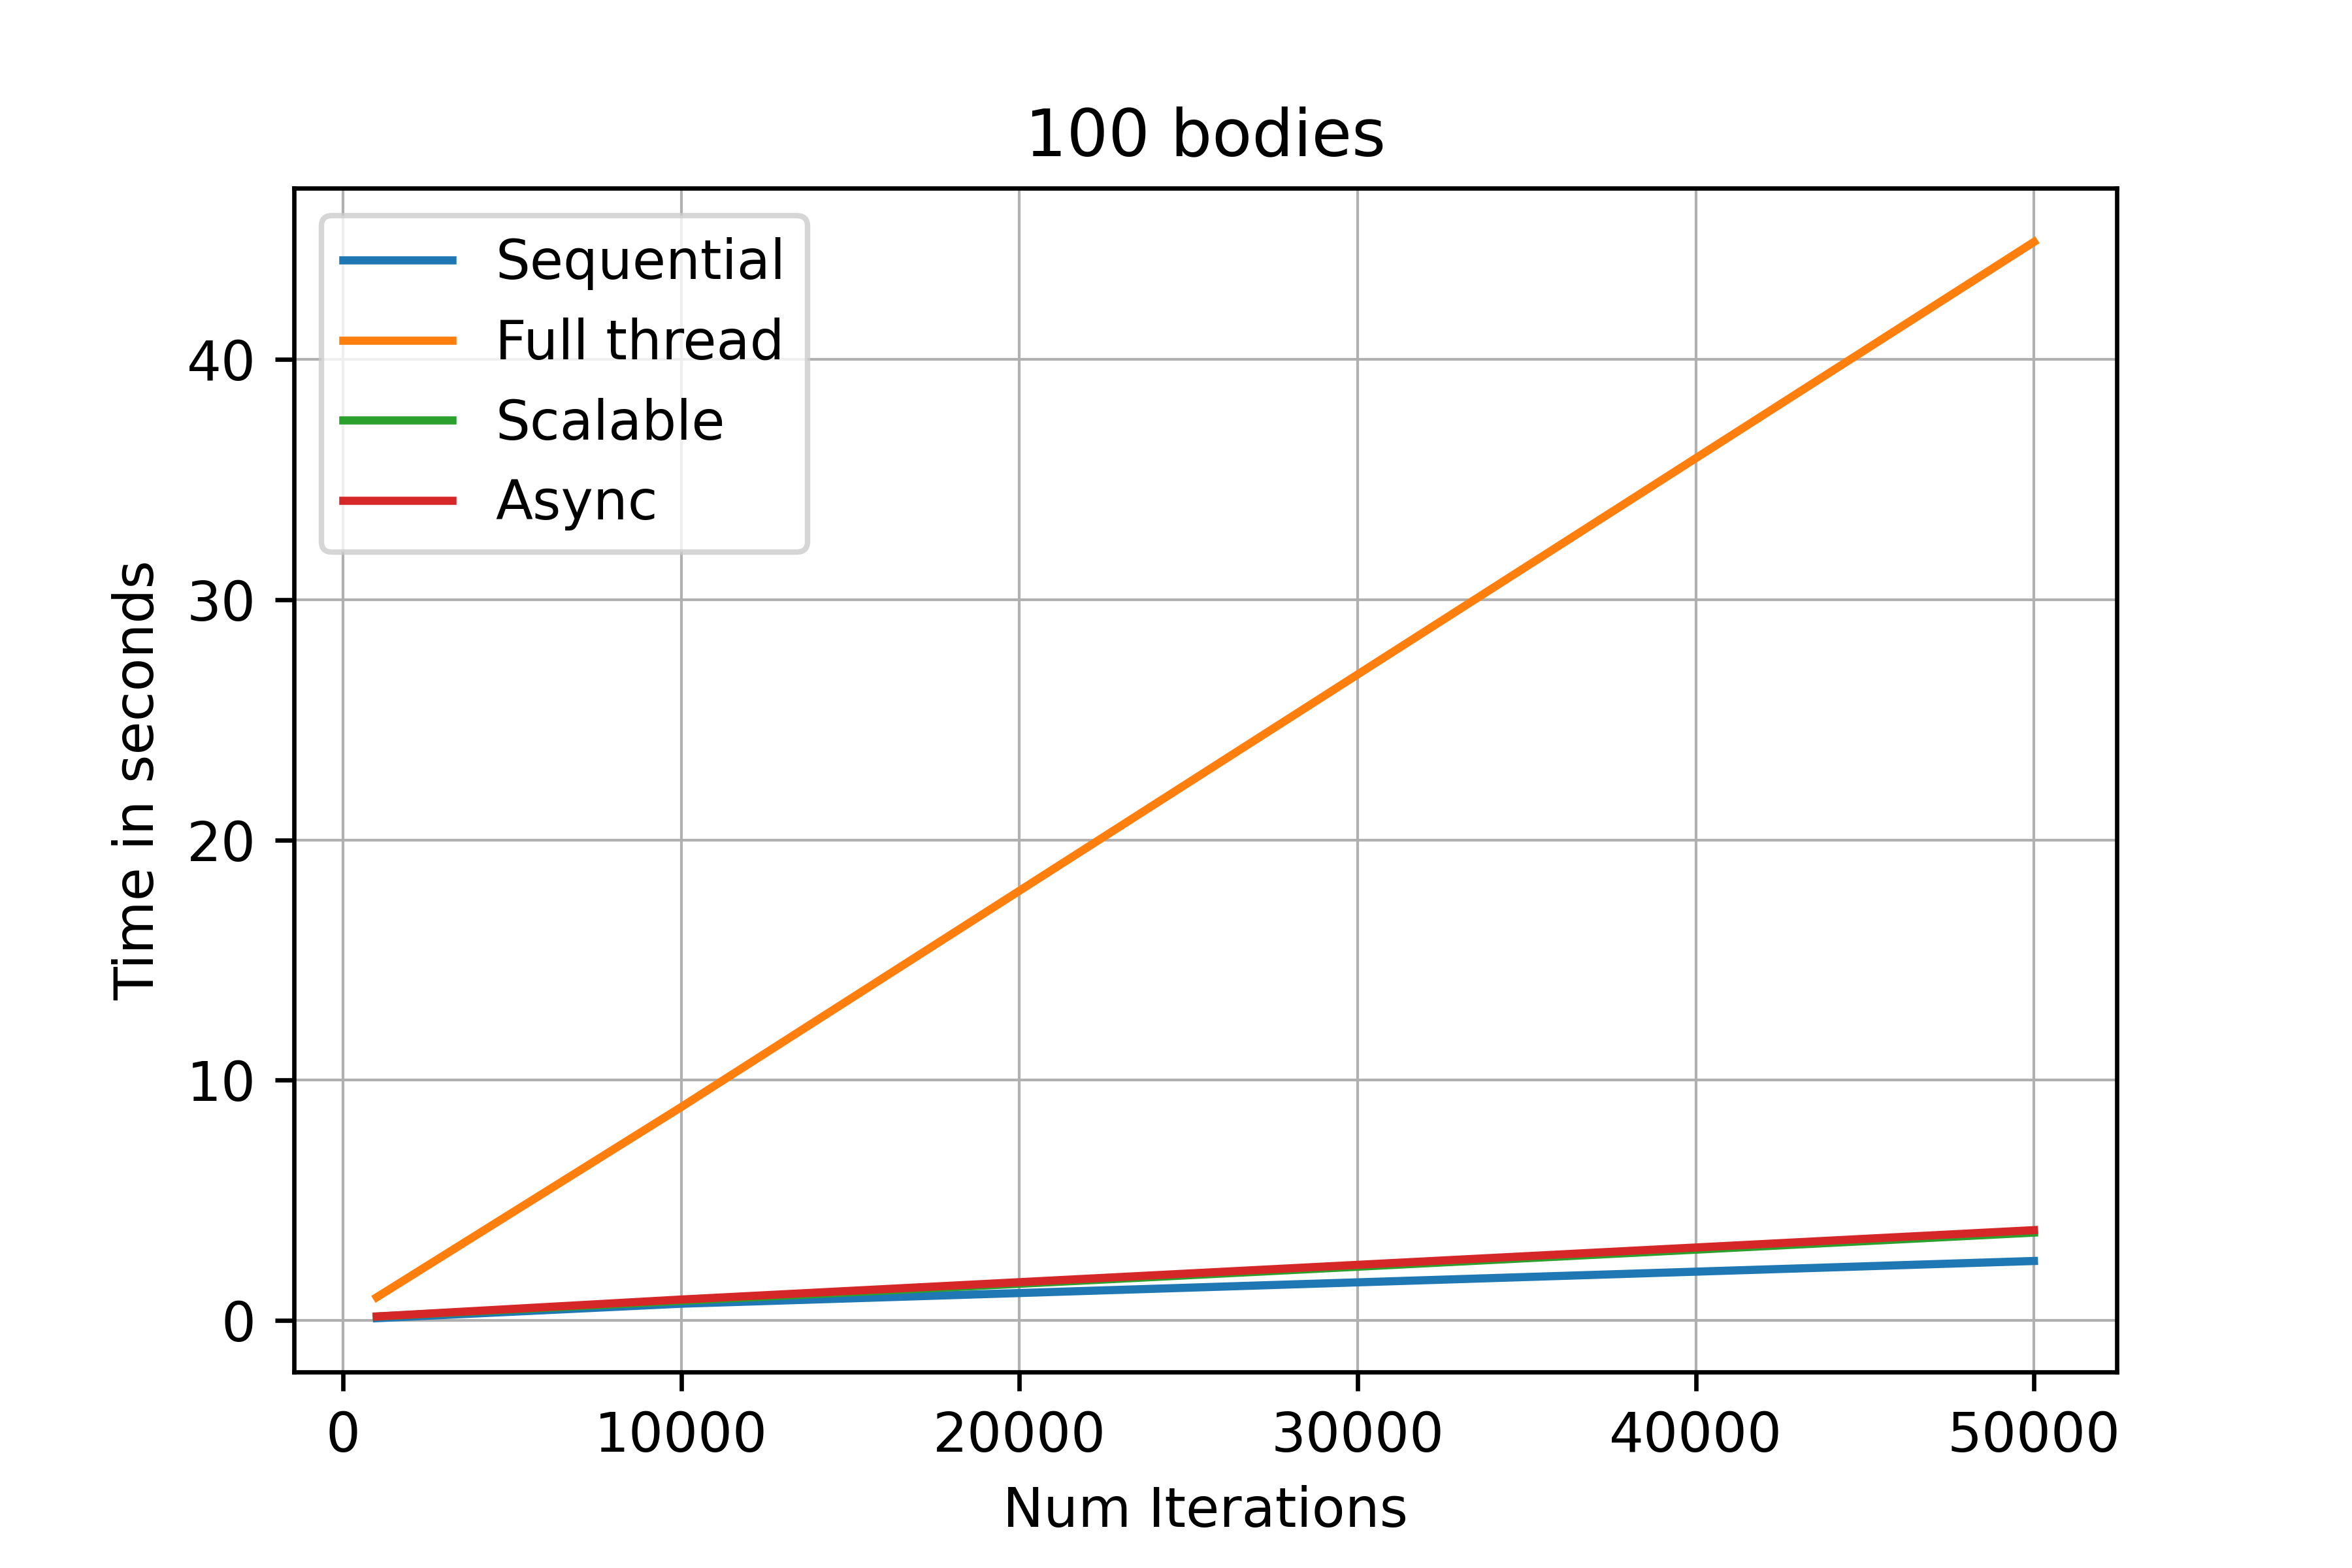
\includegraphics[scale=.45]{img/100bodies.png}}
        \end{minipage}%
        \begin{minipage}{.5\linewidth}
            \centering
            \subfloat[]{\label{stats_iterations:b}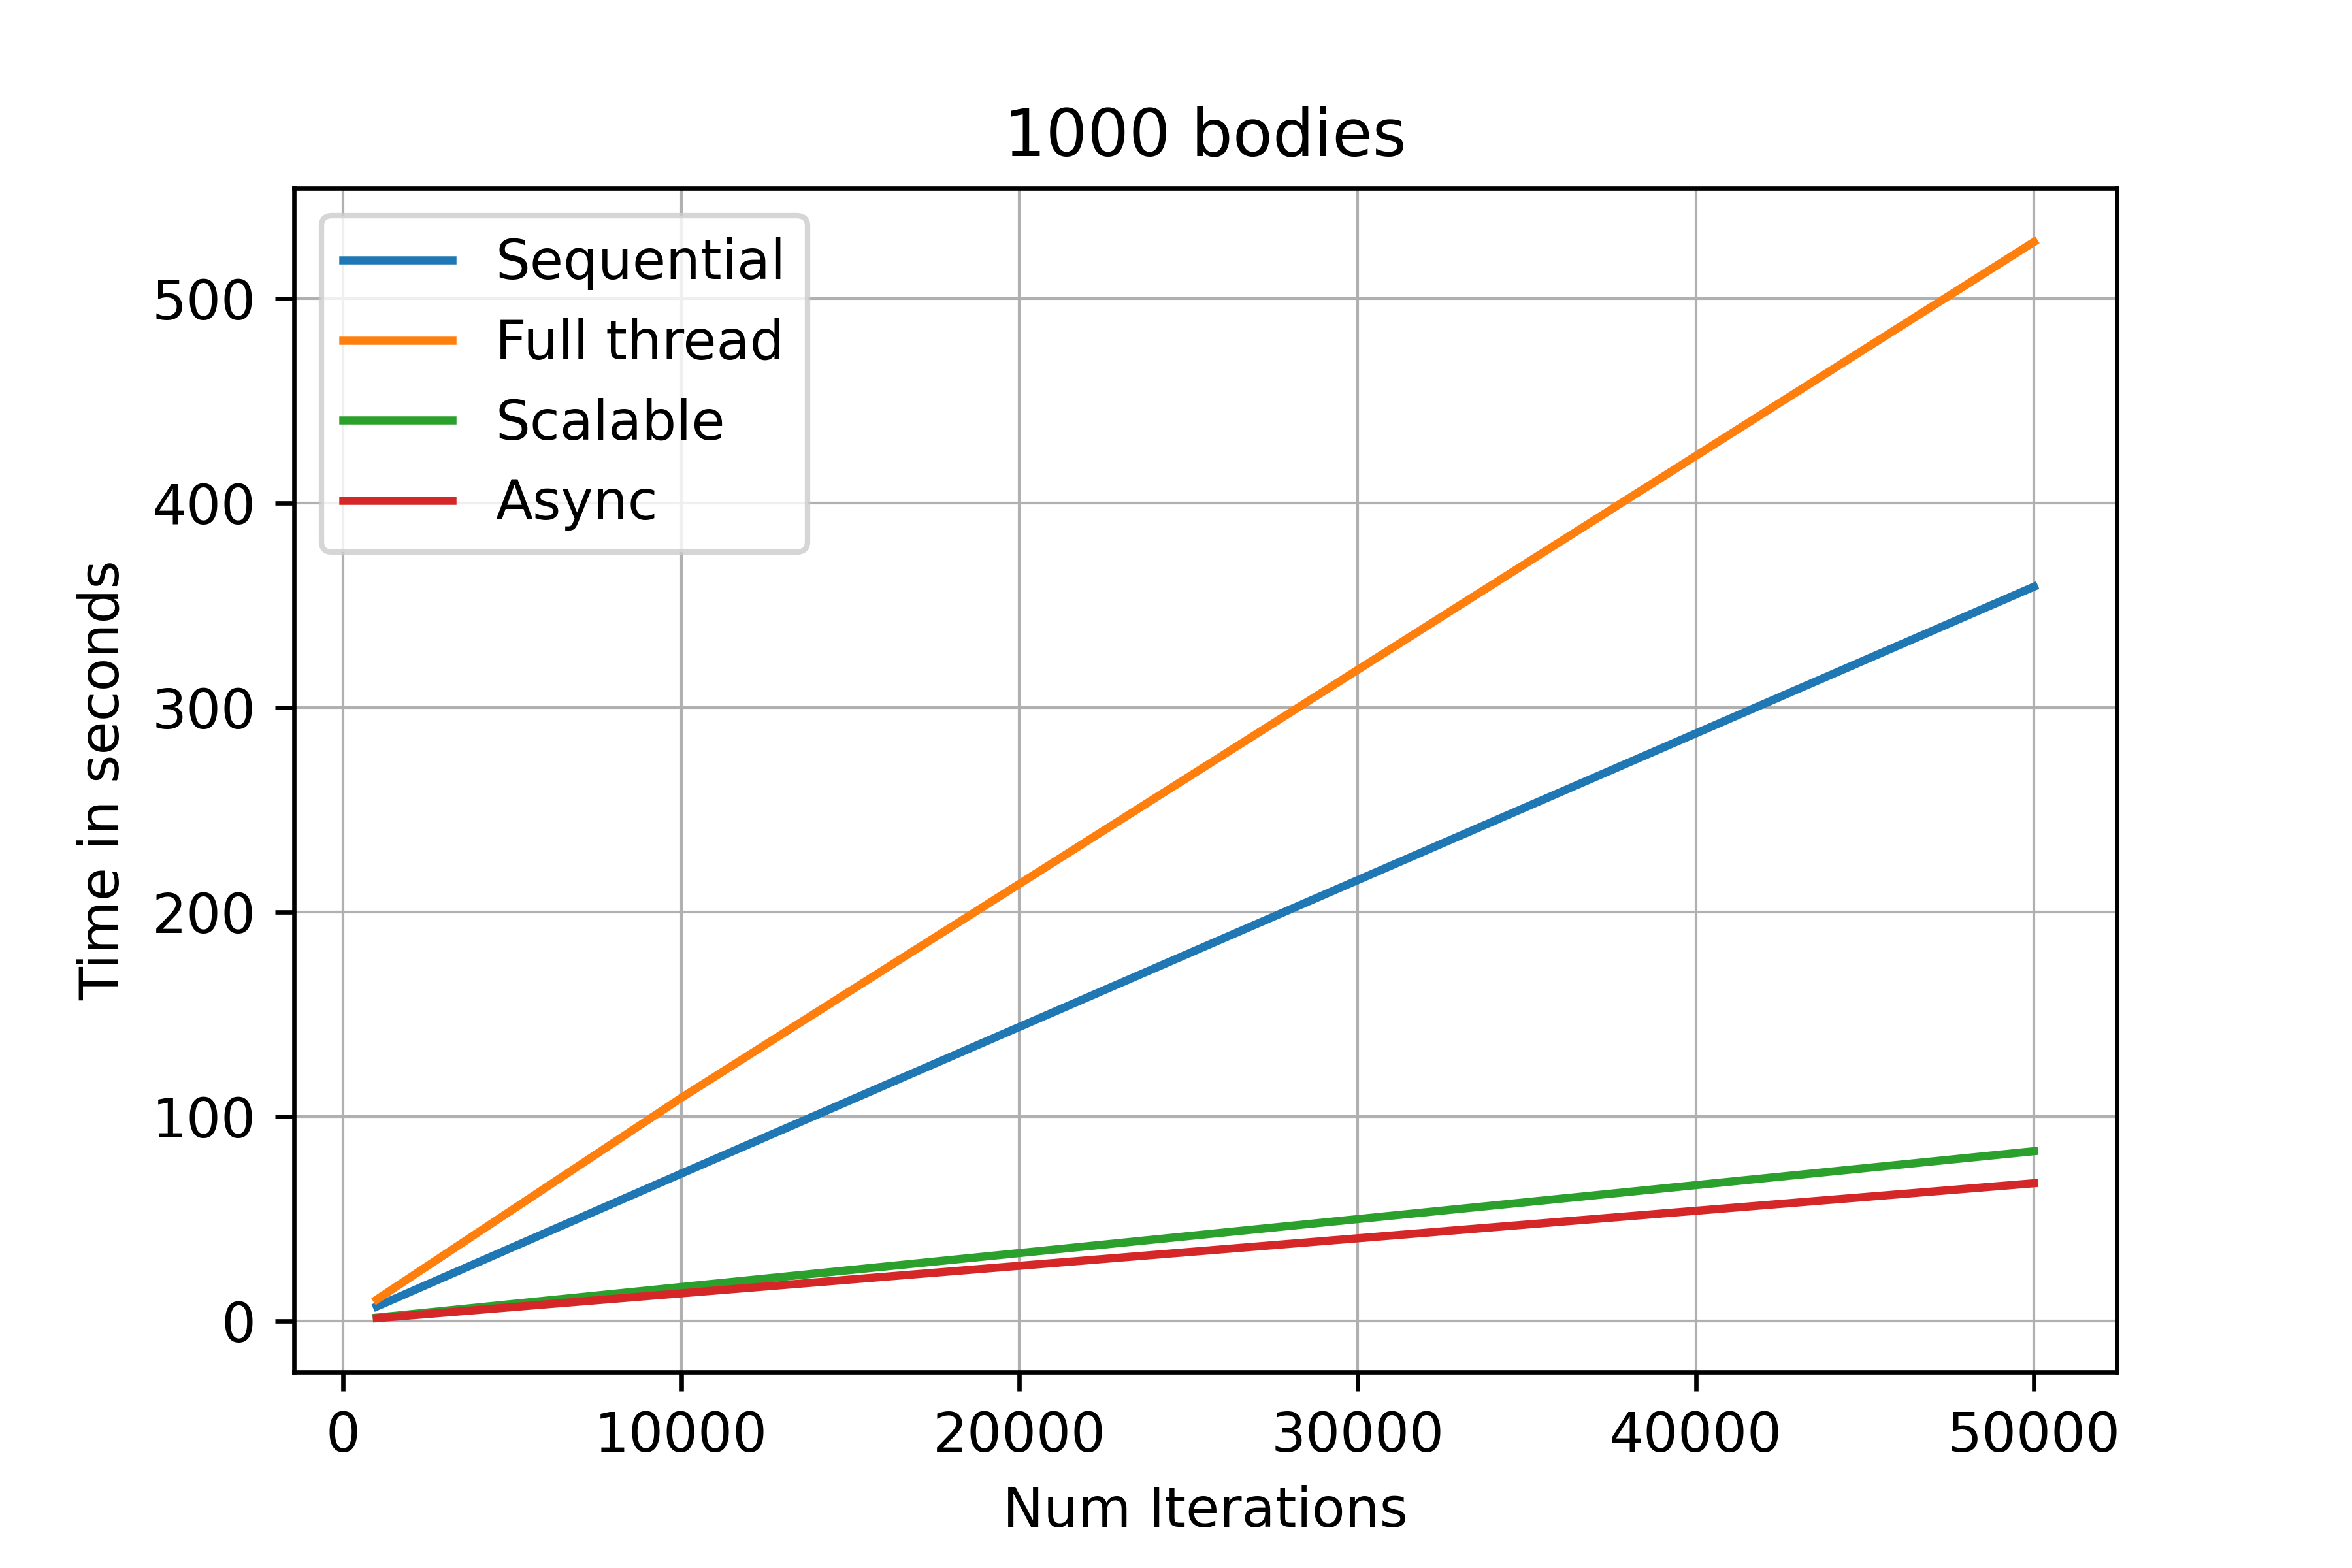
\includegraphics[scale=.45]{img/1000bodies.png}}
        \end{minipage}\par\medskip
        \subfloat[]{\label{stats_iterations:c}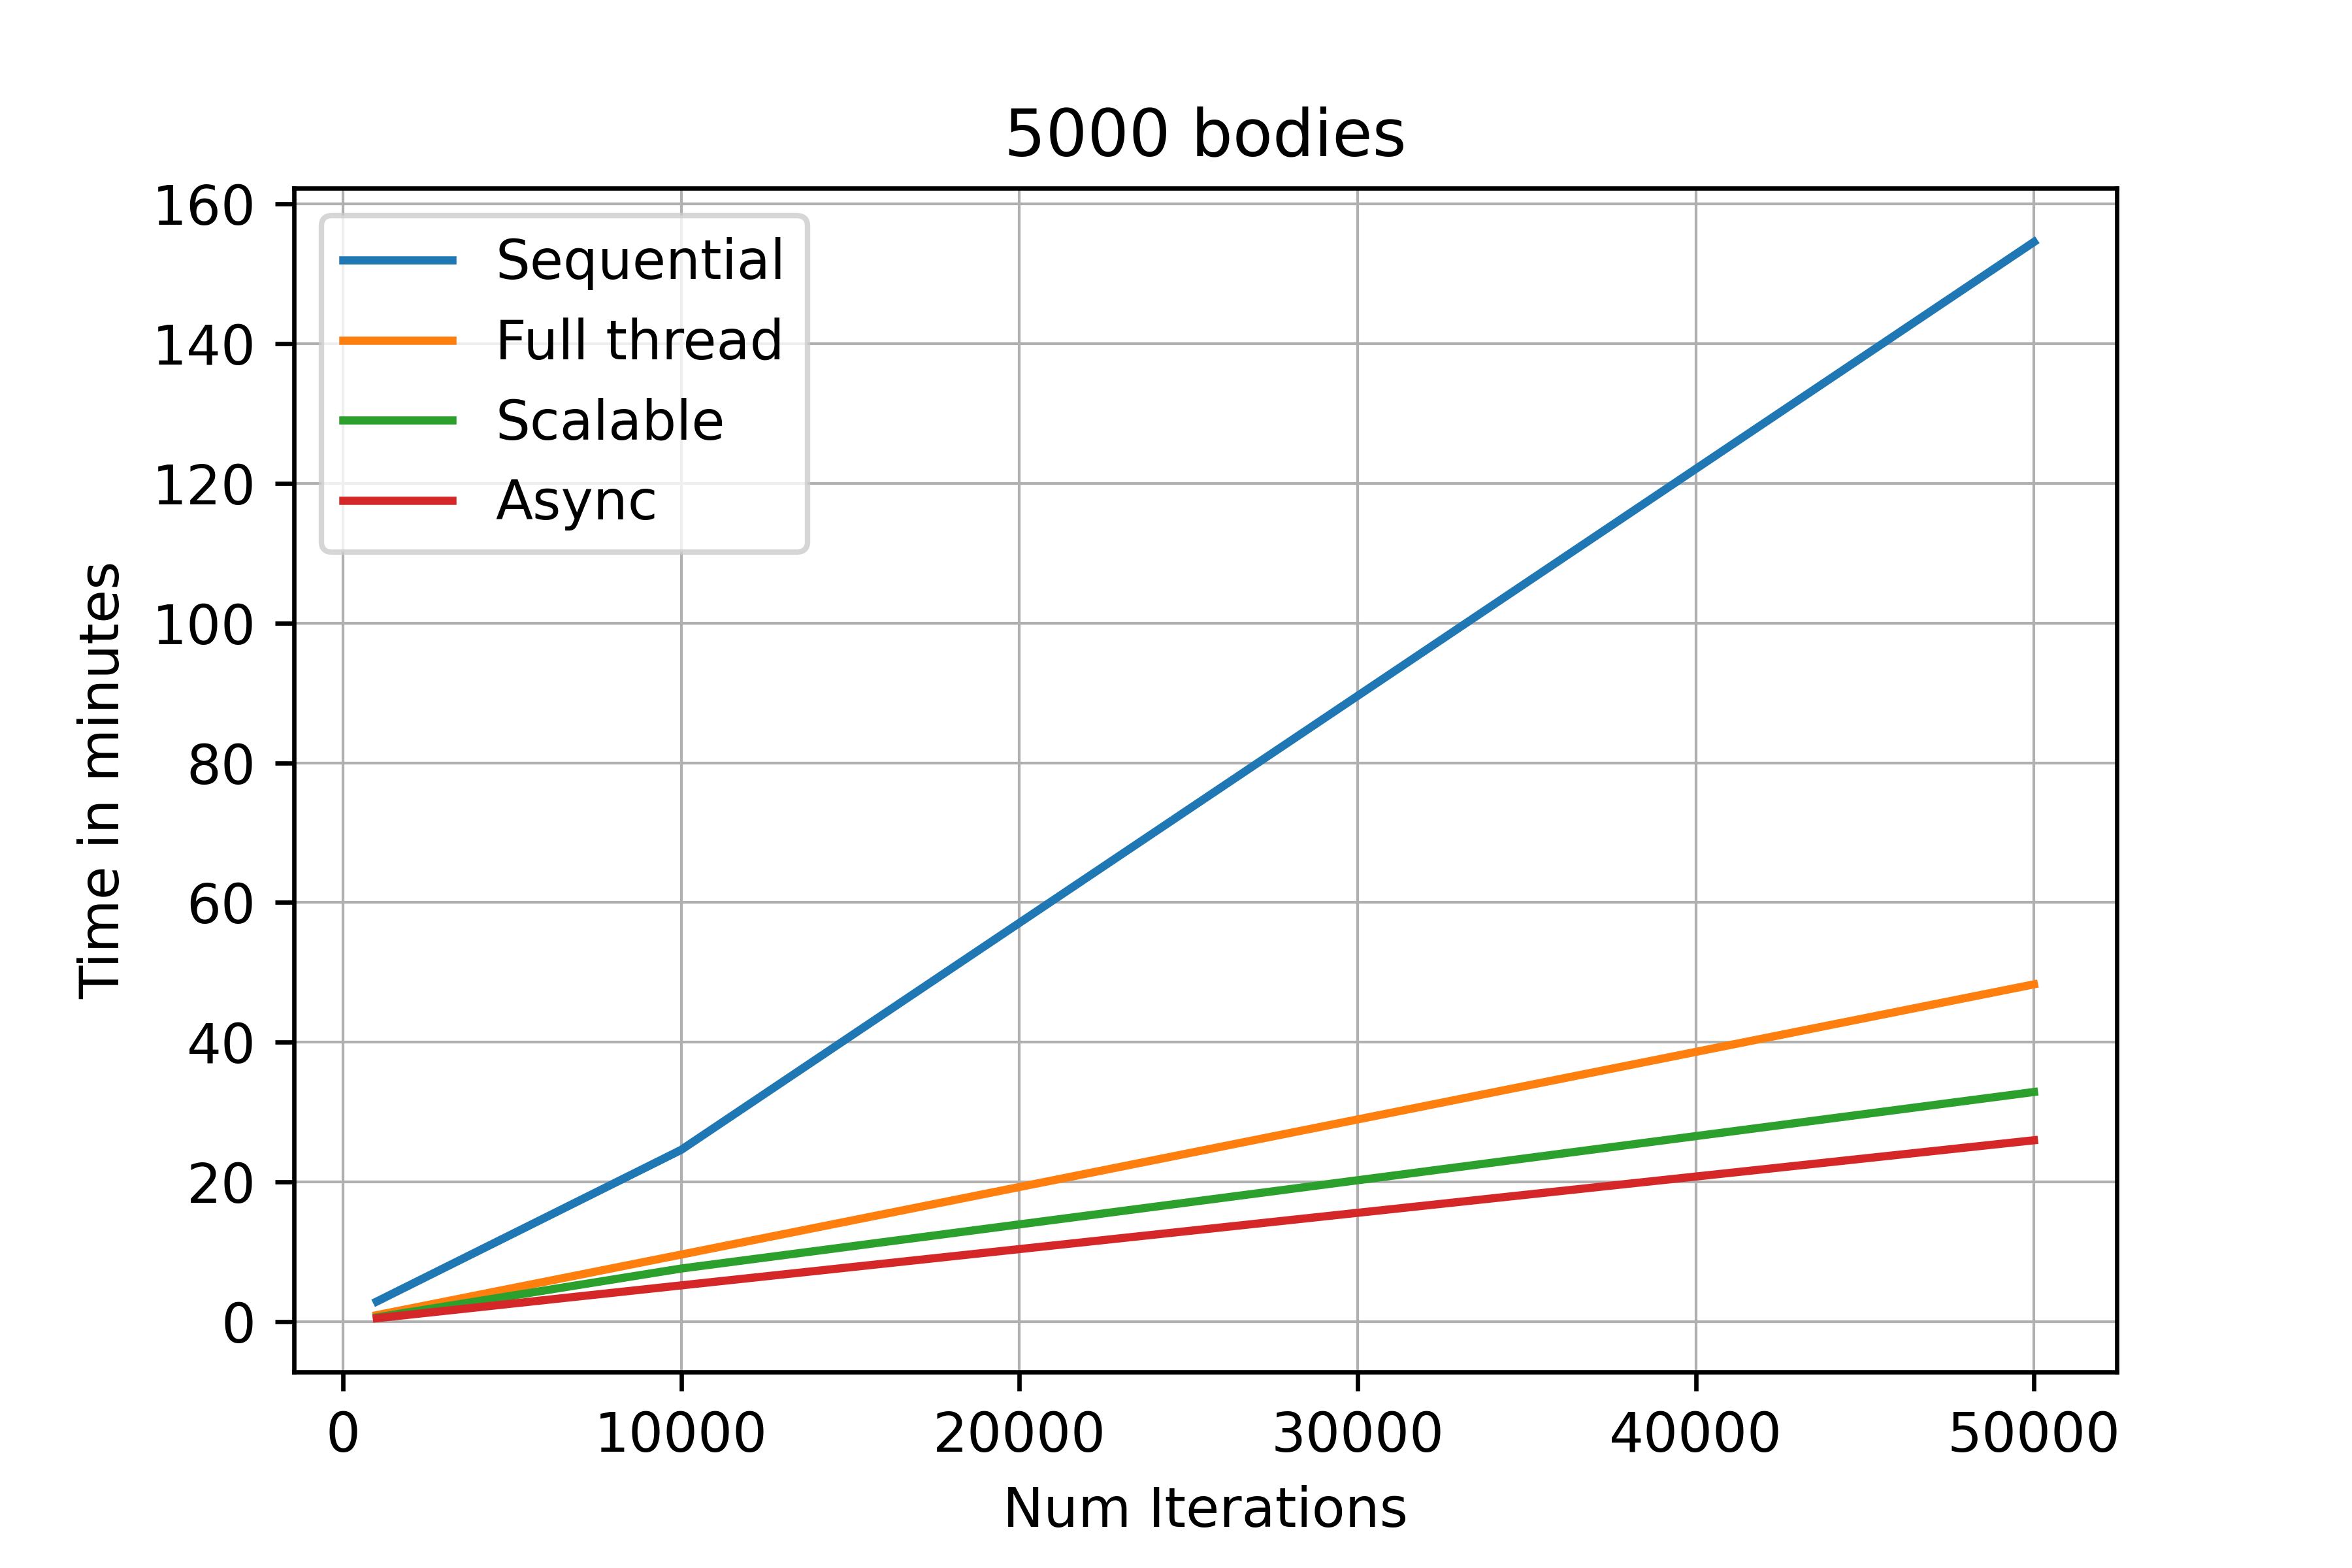
\includegraphics[scale=.5]{img/5000bodies.png}}
        \centering
        \caption{Prestazioni al variare delle iterazioni}
        \label{fig:iterations}
    \end{center}
\end{figure}

\begin{figure}[ht]
    \begin{center}
        \begin{minipage}{.5\textwidth}
            \centering
            \subfloat[]{\label{stats_bodies:a}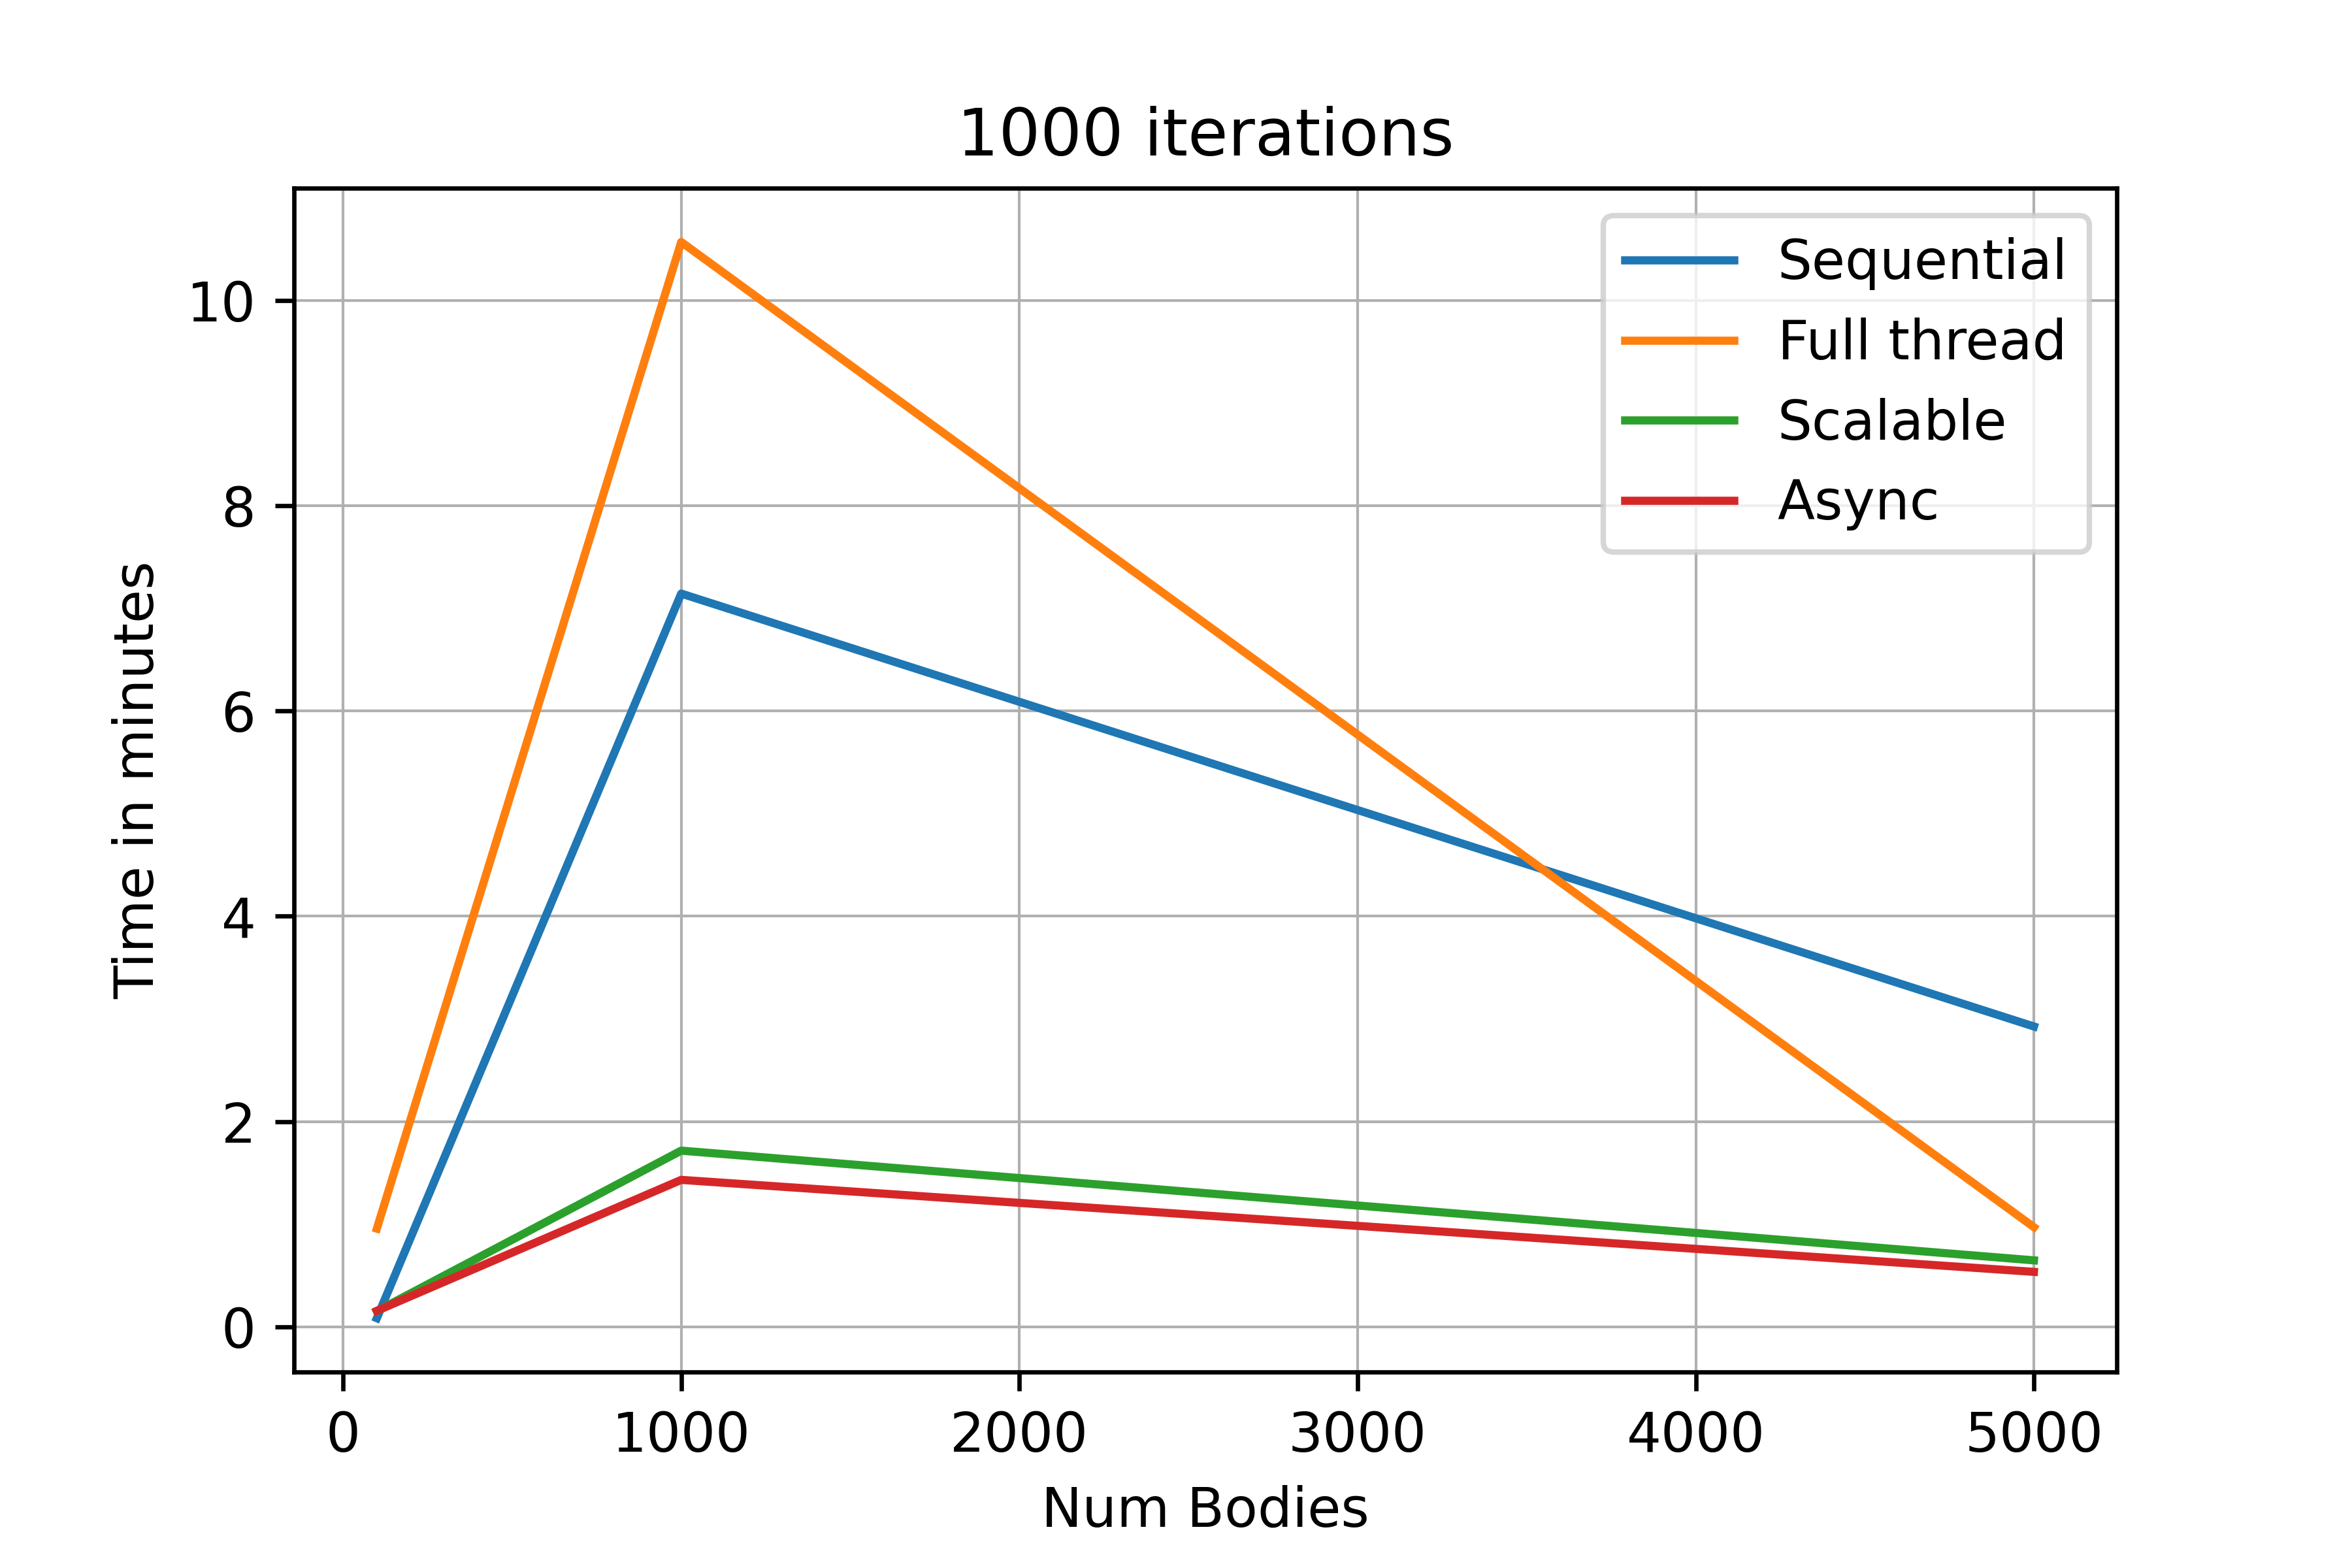
\includegraphics[scale=.45]{img/1000iterations.png}}
        \end{minipage}%
        \begin{minipage}{.5\textwidth}
            \centering
            \subfloat[]{\label{stats_bodies:b}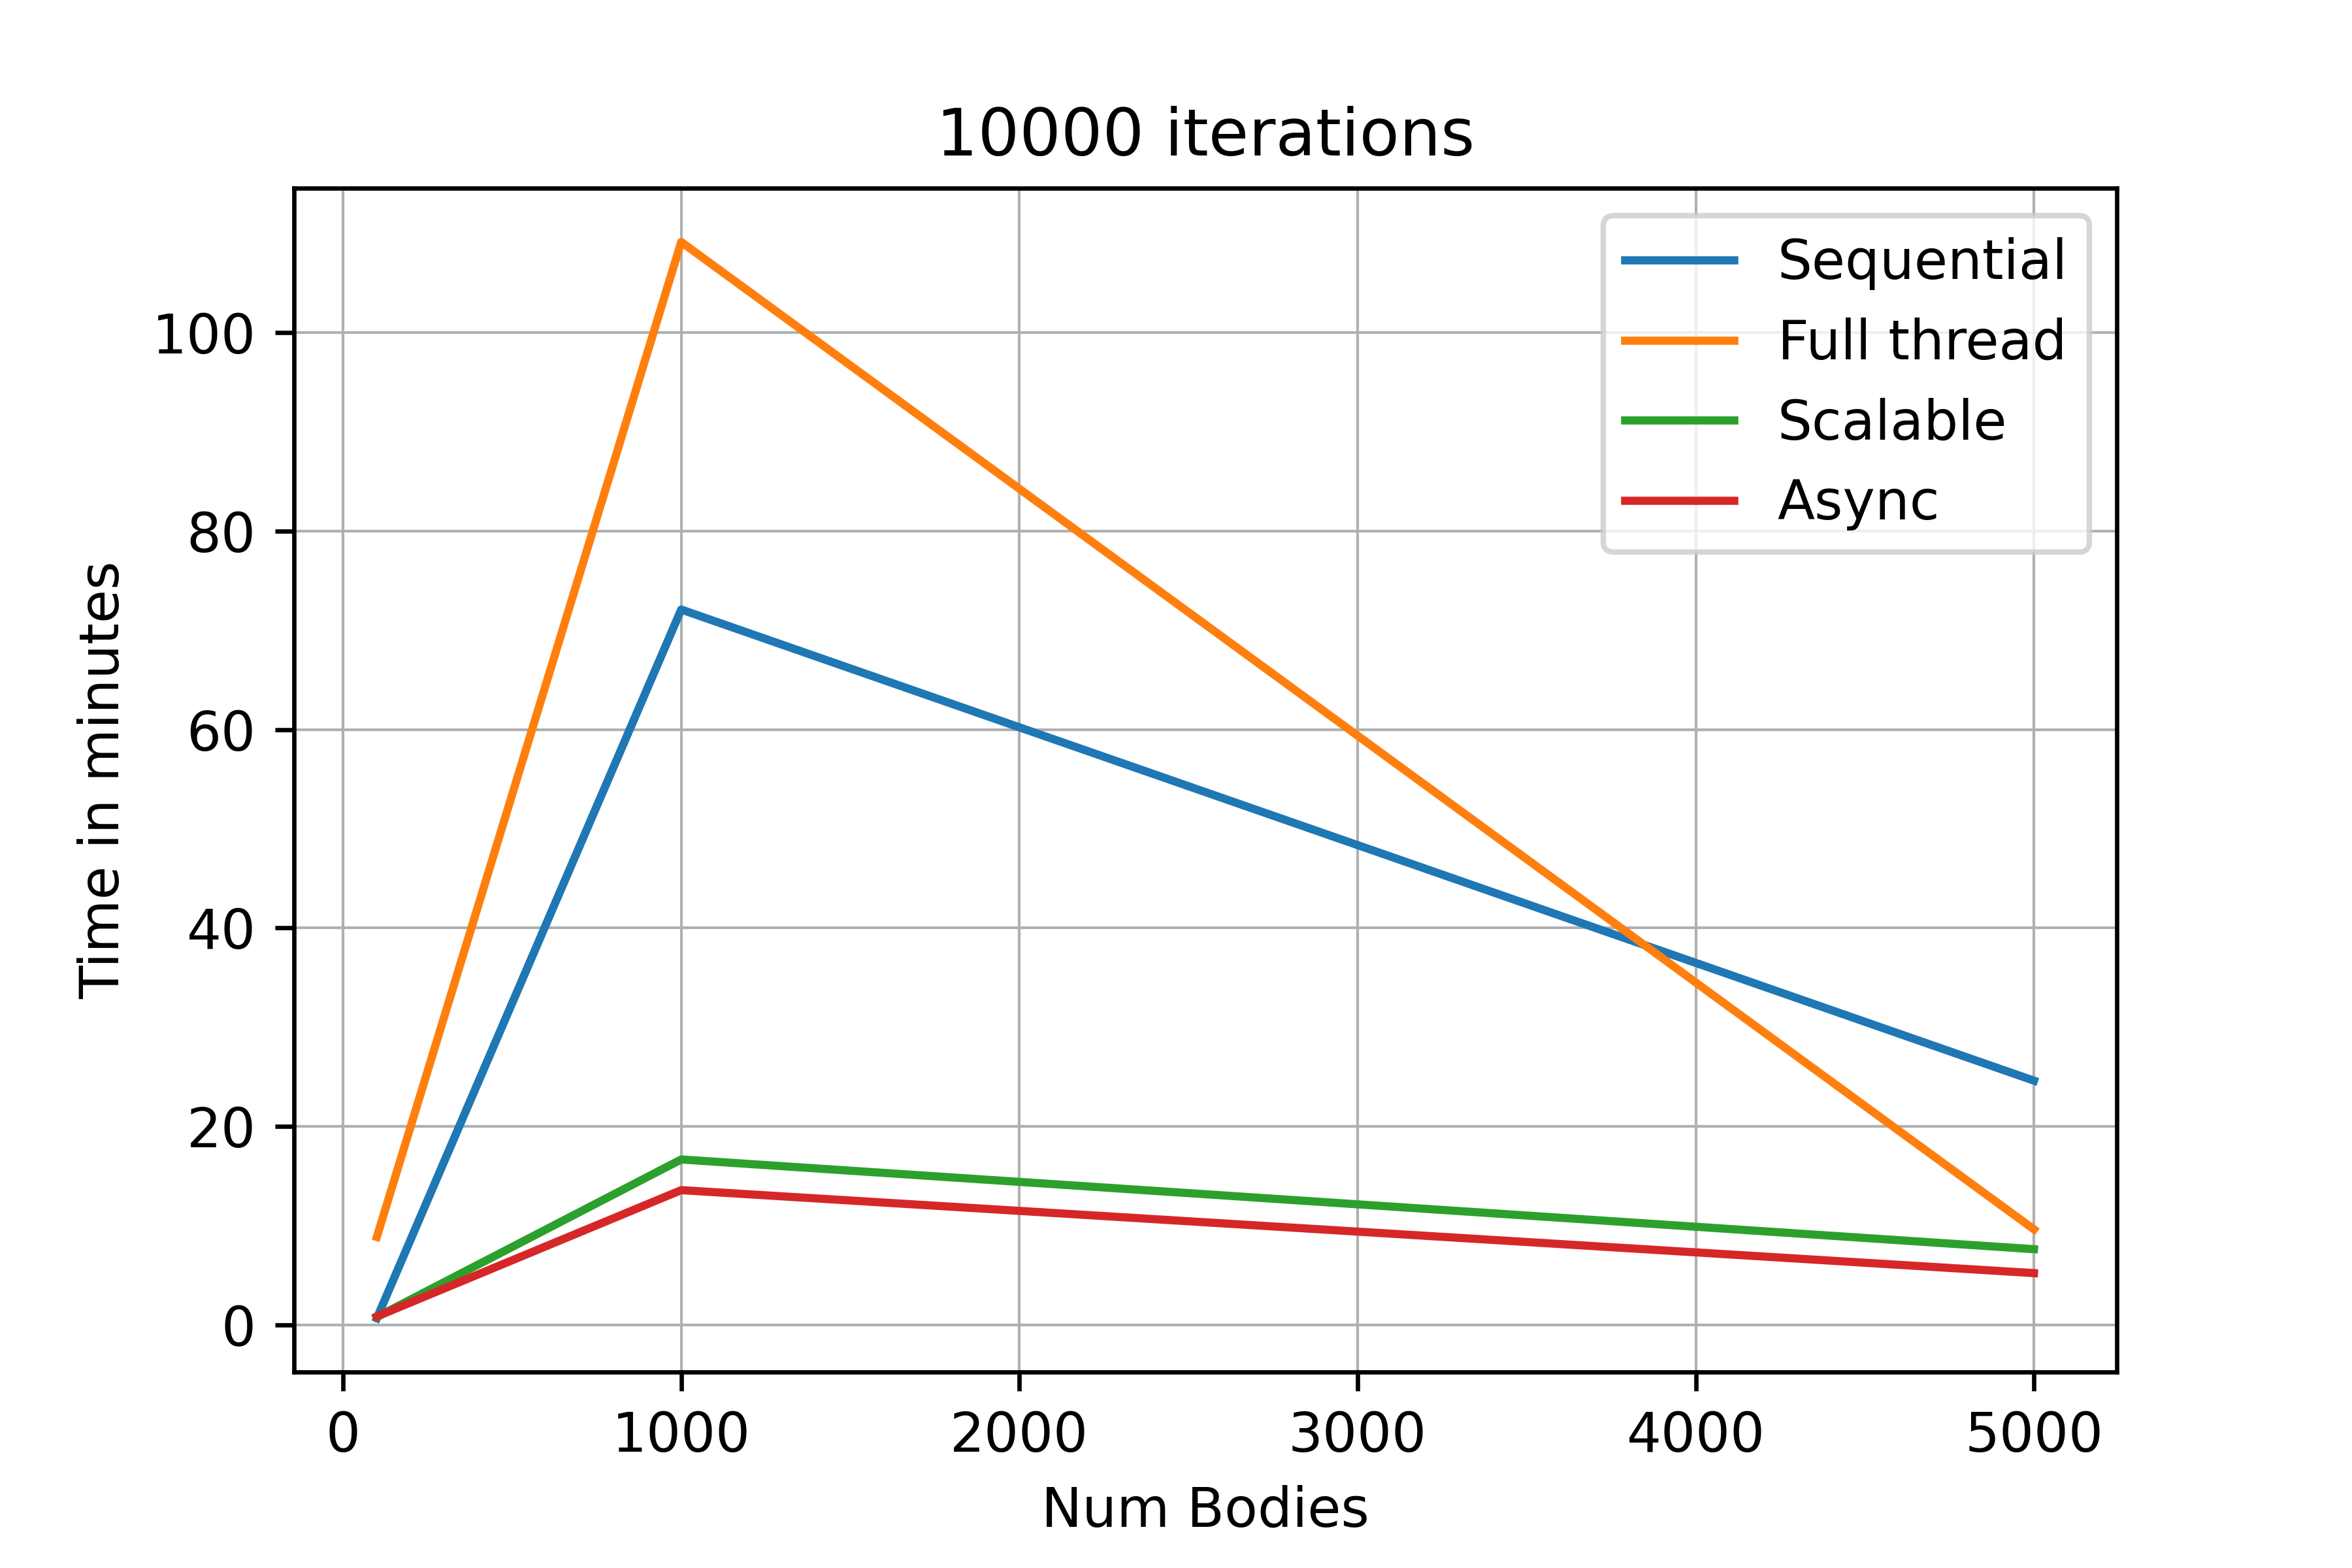
\includegraphics[scale=.45]{img/10000iterations.png}}
        \end{minipage}\par\medskip
        \subfloat[]{\label{stats_bodies:c}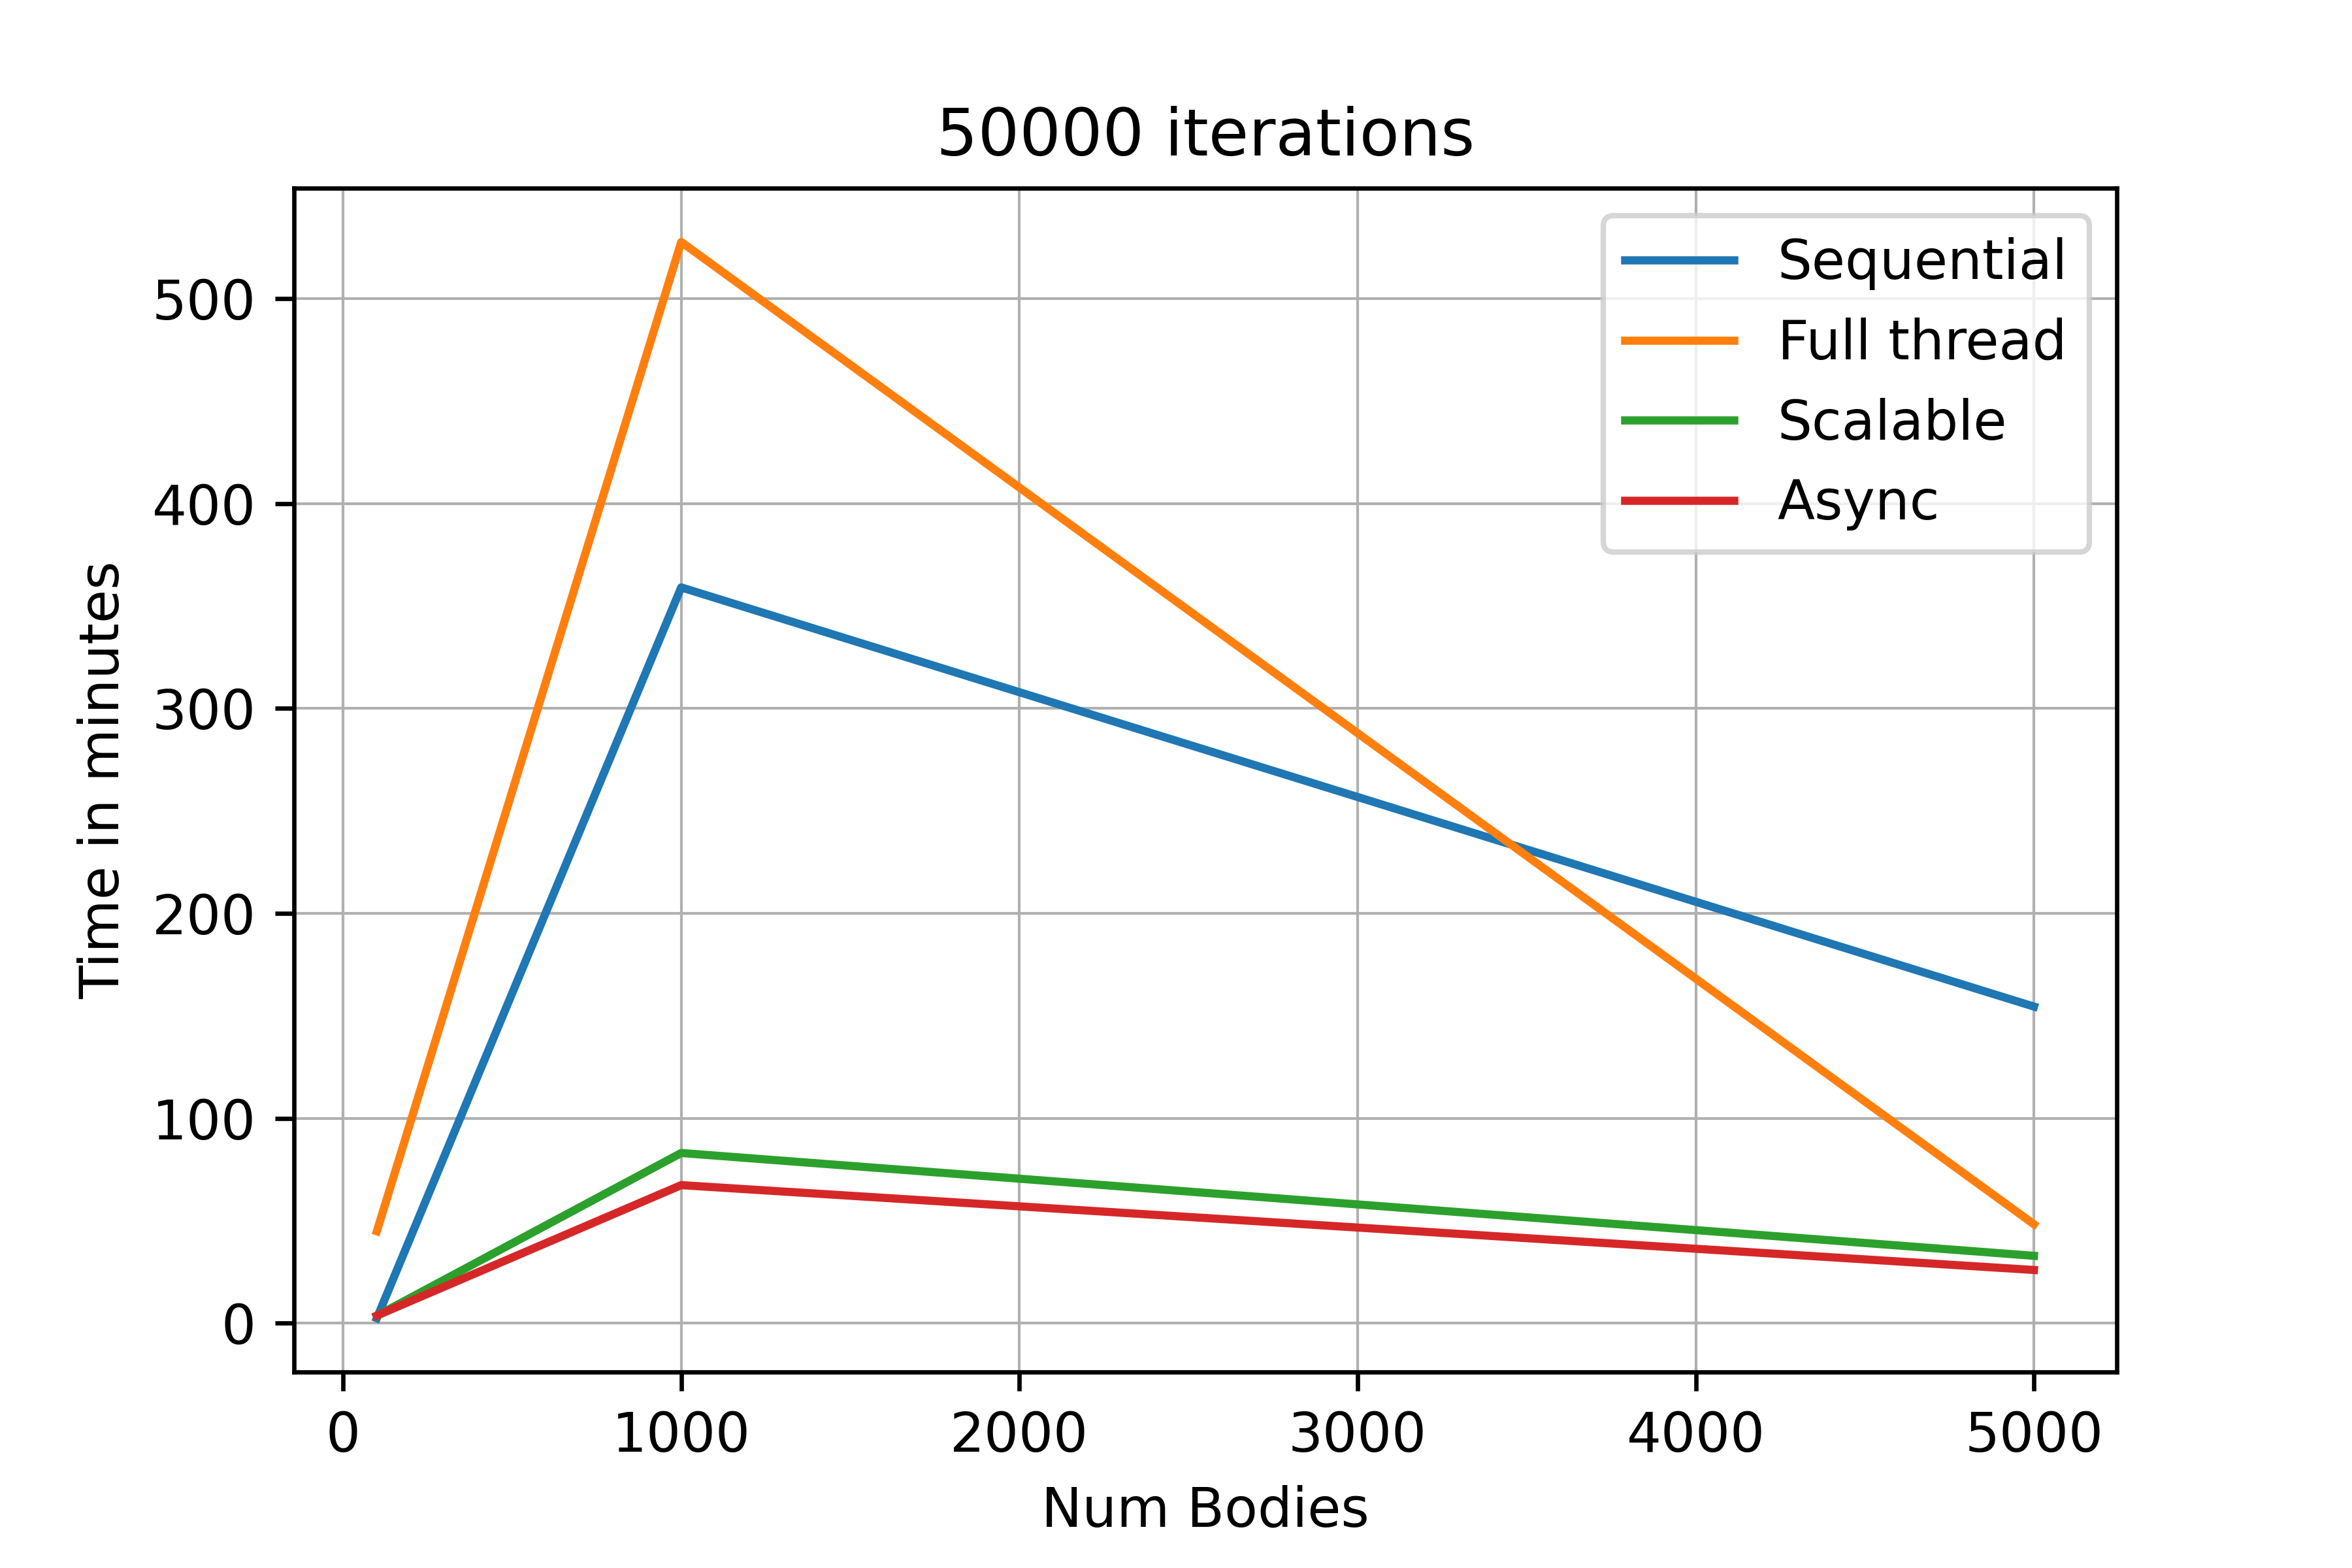
\includegraphics[scale=.5]{img/50000iterations.png}}
        \centering
        \caption{Prestazioni al variare del numero di corpi}
        \label{fig:bodies}
    \end{center}    
\end{figure}

%

\chapter{Secondo esercizio} 
\label{chapter:es2}
\section{Analisi del problema}

Si vuole implementare una libreria che metta a disposizione una serie di funzionalità minimali per l'analisi di un progetto sviluppato utilizzando il linguaggio Java.
%
Le funzionalità fornite dalla libreria devono dar la possibilità di:

\begin{enumerate}
    \item Analizzare un'interfaccia, restituendo il nome stesso e un elenco dei nomi dei metodi contenuti al suo interno.
    
    \item Analizzare una classe, restituendo il suo nome e un elenco dei metodi in essa contenuti, comprensivi di alcune informazioni ritenute essenziali: nome, modificatori (public, private, ecc.) e la loro posizione all'interno del file, specificando linea di inizio e di fine.
    
    \item Analizzare un package, riportando un analisi delle interfacce e delle classi al suo interno.
    
    \item Analizzare il progetto stesso, riportando un'analisi dei suoi package.
\end{enumerate}

Queste analisi si possono considerare a cascata, dato che le ultime si compongono di quelle precedenti.

Ulteriore requisito è quello di realizzare la libreria in modo asincrono, utilizzando un event-loop come architettura di riferimento.
%
In questo modo sarà possibile utilizzare la libreria in modo non bloccante, grazie al meccanismo delle \textit{Future}.

Inoltre, deve essere possibile poter interrompere in qualsiasi momento l'esecuzione di un'analisi precedentemente richiesta.

Infine, si intende realizzare una semplice applicazione provvista di GUI per poter testare le funzionalità messe a disposizione dalla libreria mostrando a schermo i risultati delle varie analisi.

\section{Strategia risolutiva}

La soluzione implementata, come specificato nei requisiti, si basa su programmazione asincrona in cui le varie operazioni vengono eseguite tramite l'utilizzo di un event-loop.
%
Per realizzare questo comportamento si è utilizzato il \textit{framework} \textit{Vertx}, che permette appunto di realizzare funzionalità asincrone in modo semplice, senza doversi preoccupare di molti aspetti di basso livello, come l'utilizzo effettivo dei \textit{Thread}.

Per quanto riguarda l'analisi degli elementi di un progetto Java si è utilizzato la libreria \textit{Java Parser}, che permette di creare degli \textit{Abstract Sintaxt Tree} (AST) a partire da un file .java e visitare i sui nodi per recuperare le informazioni di interesse.
%
Nello specifico, la visita viene effettuata tramite dei \textit{Visitor} in cui è possibile specificare il comportamento da adottare quando viene visitato un certo tipo di nodo.

Utilizzo di un \textit{event-loop} esterno che dovrà gestire i vari eventi che nel nostro caso sono le chiamate ai metodi per ottenere un determinato report.

La funzionalità analyzeProject lancerà una serie di eventi in base al tipo di file che si incontra durante la visita del progetto, ognuno dei quali relativo ad un certo report.

Si pensa ad una possibile soluzione in cui per ogni report si va a creare un event-loop personale in cui gestire i singoli elementi da analizzare. Tale soluzione diventa interessante se si riuscisse a fare in modo che l'event-loop generale avvia un event-loop figlio per ottenere un certo report e poi va a gestire un altro evento (la richiesta di un altro report). Deve essere l'event-loop figlio a comunicare di aver terminato al padre per fargli raccogliere il risultato. 

\section{Architettura ed implementazione}

I metodi getReport devono essere asincroni quindi tornano una Future del tipo relativo al report che si vuole ottenere (per esempio Future<ClassReport>)

\chapter{Terzo esercizio} 
\label{chapter:es3}
\input{chapter_es3}


\chapter*{Conclusioni}
\addcontentsline{toc}{chapter}{Conclusioni}

Conclusioni here.

\end{document}